\subsection{Asymptotic approximation}
Eq\ref{eq:explicitL} can be annoying to work with, especially for large $h$, so an approximation for the case $h \gg m$ is needed. Intuitively the length of a fight should have linear dependency on hitpoints as $h \rightarrow \infty$. This is because on average one can expect each hit to do $am/2$ damage and therefore it should take approximately $2h/am$ hits to kill an enemy with $h$ hitpoints. Due to overkill however, the last hit will tend to do slightly less than $am/2$ damage introducing a constant correction term to this linear approximation. We will now determine the magnitude of this constant by finding the asymptotic expansion for $\E{L_h}$.

To study the asymptotics we return to the generating function (eq\ref{eq:ogf}) and inspect its poles: the points at which it ceases to be analytic. Since the generating function is a rational function its poles are simply the zeros of the denominator
\begin{align}
	D(z) = m - (m+1)z + z^{m+1}\label{eq:denominator}.
\end{align}
According to the fundamental theorem of algebra the denominator (eq\ref{eq:denominator}) has exactly $m+1$ zeros, some of which might be duplicates.

Notice that the point $z=1$ is a zero of the denominator as $D(1) = 0$. Thus, we separate the $(z-1)$ factors writing the generating function in the form
\begin{align}
	g(z) &= \frac{(m+1)z}{{(z-1)}^2 Q(z)},
	\quad\mbox{where}\quad Q(z) = \sum_{i=0}^{m-1} (m-i) z^i.
\end{align}
We see that the generating function has a 2nd order pole at $z=1$. This allows expressing it as a partial fraction of the form
\begin{align}
	g(z) &= \frac{\alpha}{{(z-1)}^2} + \frac{\beta}{z-1} + P(z)
\end{align}
where $P(z)$ is a function that is analytic at $z=1$ and the constants $\alpha$ and $\beta$ are given by
\begin{align}
	\alpha
		&= \lim\limits_{z \rightarrow 1}{(z-1)}^2 g(z)
		 = \lim\limits_{z \rightarrow 1} \frac{(m+1)z}{Q(z)}
		 = \frac{m+1}{Q(1)}\label{eq:alphamid}\\
	\beta
		&= \lim\limits_{z \rightarrow 1}\frac{\d}{\d z}\Big({(z-1)}^2 g(z)\Big)
		 = \lim\limits_{z \rightarrow 1} \frac{m+1}{Q(z)}\left(1 - \frac{zQ'(z)}{Q(z)}\right)
		 = \alpha\left(1 - \frac{Q'(1)}{Q(1)}\right)\label{eq:betamid}.
\end{align}
The values of the polynomial $Q(z)$ and its derivative $Q'(z)$ at $z=1$ can be computed to be
\begin{align}
	Q(1)
		&= \sum_{i=0}^{m-1} (m-i)
		 = \frac{m(m+1)}{2}\\
	Q'(1)
		&= \sum_{i=1}^{m-1} i(m-i)
		 = \frac{m(m+1)(m-1)}{6}.
\end{align}
Substituting them back into eq\ref{eq:alphamid} and eq\ref{eq:betamid} yields $\alpha = \frac{2}{m}$ and $\beta = \frac{4-m}{3m}$. Now we continue with the partial fraction form of the generating function and expand the first two terms as a power series around $z=0$.
\begin{align}
	g(z)
		&= \frac{2}{m}\frac{1}{{(z-1)}^2} + \frac{4-m}{3m}\frac{1}{z-1} + P(z)\\
		&= \frac{2}{m}\left(\frac{\d}{\d z}\Big(\frac{1}{1-z}\Big) + \frac{m-4}{3}\frac{1}{1-z}\right) + P(z)\\
		&= \frac{2}{m}\bigg(\frac{\d}{\d z}\sum_{n=0}^\infty z^n + \frac{m-4}{3}\sum_{n=0}^\infty z^n\bigg) + P(z)\\
		&= \frac{2}{m}\bigg(\sum_{n=1}^\infty n z^{n-1} + \sum_{n=0}^\infty \frac{m-4}{3}z^n\bigg) + P(z)\\
		&= \frac{2}{m}\bigg(\sum_{n=0}^\infty (n+1) z^n + \sum_{n=0}^\infty \frac{m-4}{3}z^n\bigg) + P(z)\\
		&= \sum_{n=0}^\infty \frac{2}{m}\Big(n + \frac{m - 1}{3}\Big) z^n + P(z)\\
\end{align}

\begin{align}\label{eq:asymptoticAppr}
\langle L_h \rangle \sim \frac{2}{ma}\left(h + \frac{m-1}{3}\right)
\end{align}
The correctness of both the explicit solution and the asymptotic approximation were verified by comparing them to a computer simulation. The comparison is illustrated in figure~2.
\begin{figure}[t]\label{fig:apprComparison}
    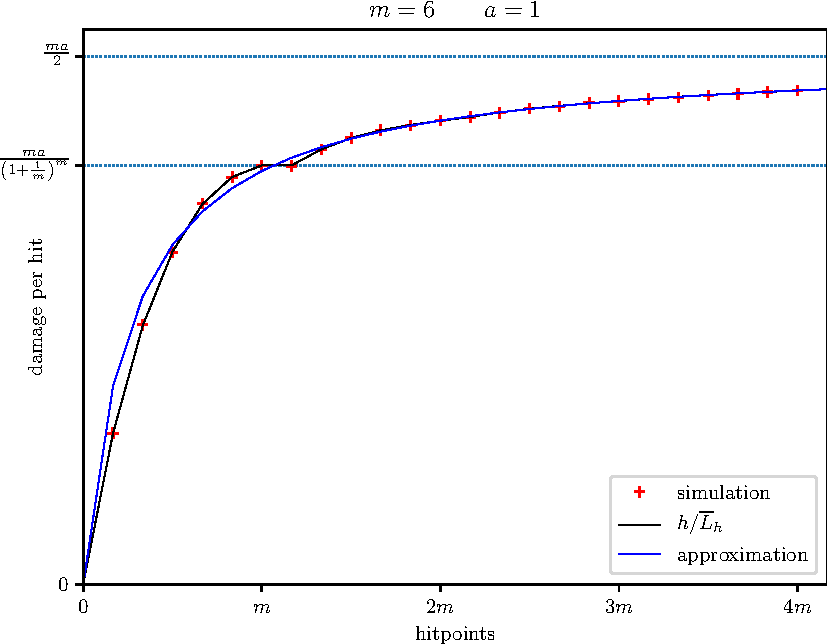
\includegraphics[scale=1.1]{dph-appr-m6.pdf}
    \caption{Comparison of damage per hit (DPH) calculated using the explicit formula (eq\ref{eq:explicitL}), asymptotic approximation (eq\ref{eq:asymptoticAppr}) and a simulation. The simulation was written using the damage calculation mechanics described in Chapter~\ref{chap:fightDef}. For each datapoint $10^{5}$ fights were simulated and their average lengths calculated.}
\end{figure}
